\documentclass{beamer}

\mode<presentation> {

\usetheme{Frankfurt}

}

\definecolor{darkblue}{RGB}{0,0,90}

\setbeamercolor{date in head/foot}{fg=white,bg=black}
\setbeamercolor{title in head/foot}{fg=white,bg=darkblue}

\setbeamertemplate{footline}
{
  \leavevmode%
  \hbox{%
  \begin{beamercolorbox}[wd=.45\paperwidth,ht=2.25ex,dp=1ex,center]{author in head/foot}%
    \usebeamerfont{author in head/foot}\insertshortauthor\; \;| \; \insertshortdate{}
  \end{beamercolorbox}%
  \begin{beamercolorbox}[wd=.45\paperwidth,ht=2.25ex,dp=1ex,center]{title in head/foot}%
    \usebeamerfont{title in head/foot}\insertsection\hspace*{3em}
  \end{beamercolorbox}%
  \begin{beamercolorbox}[wd=.1\paperwidth,ht=2.25ex,dp=1ex,center]{date in head/foot}%
    \insertframenumber{} \hspace*{1ex}
  \end{beamercolorbox}}%
  \vskip0pt%
}

\usepackage{graphicx} % Allows including images
\usepackage{booktabs} % Allows the use of \toprule, \midrule and \bottomrule in tables

%----------------------------------------------------------------------------------------
%	TITLE PAGE
%----------------------------------------------------------------------------------------

\title[NIDS]{Intrusion Detection Systems} % The short title appears at the bottom of every slide, the full title is only on the title page

\author{Laurent De Wilde} % Your name
\institute[VUB] % Your institution as it will appear on the bottom of every slide, may be shorthand to save space
{
Vrije Universiteit Brussel \\ 
Faculty of Science and Bio - Engineering Sciences \\
Department of Computer Science \\% Your institution for the title page
\medskip
\textit{laudewil@vub.ac.be} % Your email address
}
\date{January 27, 2015} % Date, can be changed to a custom date

\begin{document}

\begin{frame}
\titlepage % Print the title page as the first slide
\end{frame}

\begin{frame}
\frametitle{Overview} % Table of contents slide, comment this block out to remove it
\tableofcontents % Throughout your presentation, if you choose to use \section{} and \subsection{} commands, these will automatically be printed on this slide as an overview of your presentation
\end{frame}

%----------------------------------------------------------------------------------------
%	PRESENTATION SLIDES
%----------------------------------------------------------------------------------------

%------------------------------------------------
\section{What is an IDS?} % Sections can be created in order to organize your presentation into discrete blocks, all sections and subsections are automatically printed in the table of contents as an overview of the talk
%------------------------------------------------

%\begin{figure}
 %  \includegraphics[width= 0.8\linewidth]{images/analyzer.png}
%\end{figure}

\subsection*{What is an IDS?}

\begin{frame}
\frametitle{What is an IDS?}
Two types of IDS exist
\begin{block}{Network IDS}
	\begin{itemize}
	\item Detects and prevents network intrusions
	\item Entire network 
	\end{itemize}
\end{block}
\begin{block}{Host IDS}
	\begin{itemize}
	\item Ensures the host integrity
	\item Single host
	\end{itemize}
\end{block}

\end{frame}

%-------------------------------------------------------------------
\section{Snort}
\subsection*{Snort}

\begin{frame}
\frametitle{Snort}
\begin{block}{What is Snort?}
	\begin{itemize}
	\item Signature-based
	\item Network IDS
	\item Free (GPLv2 license)
	\item Highly customizable
	\end{itemize}
\end{block}
\end{frame}
%--------------------------------------------------------------------
\section{Testing and configuring Snort}
\subsection*{}

\begin{frame}
\frametitle{\insertsection}
\textbf{Practical testing and configuration of Snort}
\end{frame}

\begin{frame}
\frametitle{How was Snort configured?}
By performing attacks on the network.
\begin{block}{Based on the outcome}
	\begin{itemize}
	\item Signatures were added
	\item Signatures were edited
	\item Signatures were removed
	\item Other aspects of Snort were fine-tuned
	\end{itemize}
\end{block}
\end{frame}

\begin{frame}
\frametitle{Which attacks have been executed? (1/2)}
\begin{itemize}
\item Port scans
	\begin{itemize}
	\item Basic port scan
	\item Advanced port scan
	\end{itemize}
\item Webserver attacks
	\begin{itemize}
	\item VISA card numbers sent in plain text over the network
	\item XSS
	\item SQL Injection
	\item Command Injection
	\end{itemize}
\item FTP server attacks
	\begin{itemize}
	\item FTP root access
	\item FTP malicious payloads
	\item Various other FTP attacks
	\end{itemize}
\end{itemize}
\end{frame}

\begin{frame}
\frametitle{Which attacks have been executed? (2/2)}
\begin{itemize}
\item SSH attacks
\item SMB attacks
	\begin{itemize}
	\item List shares
	\item List users
	\item Login attempts
	\item Bruteforce attempts
	\end{itemize}
\item Database attacks
	\begin{itemize}
	\item Database scanning
	\item Login attempts (including root access)
	\item Bruteforce attempts
	\end{itemize}
\item Trojan and virus injection / infection
\item DOS attacks
\end{itemize}
\end{frame}

\begin{frame}
\frametitle{First things first: basic configuration (1/5)}
Setting up the network in Linux\ldots
\begin{figure}
   \includegraphics[width= 1\linewidth]{../images/VM_network.png}
\end{figure}
\end{frame}
\begin{frame}
\frametitle{First things first: basic configuration (2/5)}
\ldots
\begin{figure}
   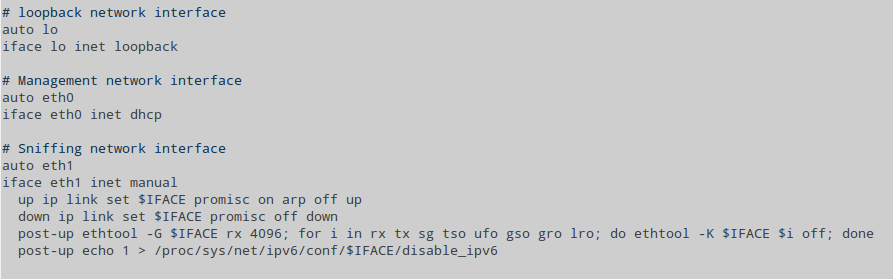
\includegraphics[width= 1\linewidth]{../images/VM_network_3.png}
\end{figure}
\end{frame}
\begin{frame}
\frametitle{First things first: basic configuration (3/5)}
\ldots as well as in snort.conf
\begin{figure}
   \includegraphics[width= 0.7\linewidth]{../images/VM_network_2.png}
\end{figure}
\end{frame}
\begin{frame}
\frametitle{First things first: basic configuration (4/5)}
Running PulledPork to update the rules.
\begin{figure}
   \includegraphics[width= 0.5\linewidth]{../images/VM_PulledPort_rules.png}
\end{figure}
\end{frame}
\begin{frame}
\frametitle{First things first: basic configuration (5/5)}
\begin{figure}
   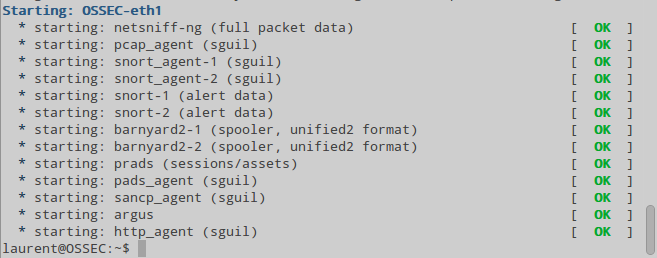
\includegraphics[width= 0.9\linewidth]{../images/VM_OK.png}
\end{figure}
\end{frame}

%------------------------------

\begin{frame}
\frametitle{Portscans - Regular}
\textbf{nmap -T4 -A -v 192.168.100.17}\\
Detected by Snort!
\begin{figure}
   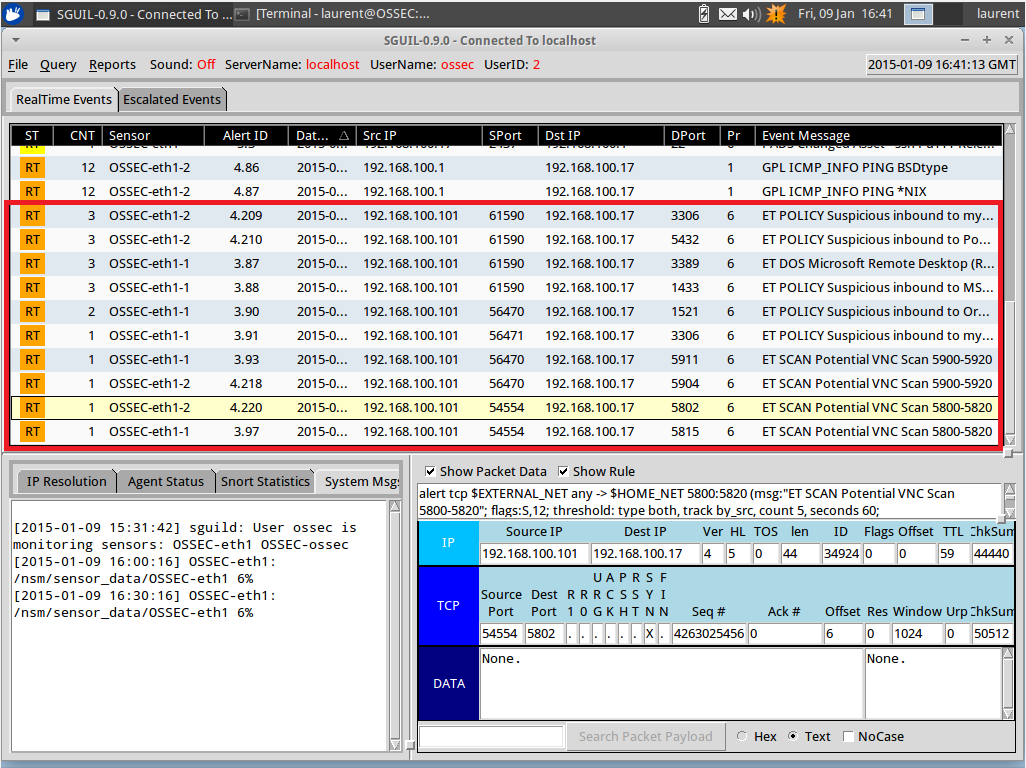
\includegraphics[width= 0.7\linewidth]{../images/VM_portscan_2.png}
\end{figure}
\end{frame}
\begin{frame}
\frametitle{Portscans - SYN}
\textbf{nmap -T4 -A -Ss -f -v 192.168.100.17}\\
Not detected $=>$ need to add some extra rules
\begin{figure}
   \includegraphics[width= 1\linewidth]{../images/VM_SynNULL_3.png}
\end{figure}
\end{frame}
\begin{frame}
\frametitle{Portscans - NULL and XMAS (1/2)}
\textbf{nmap -T4 -A -sN -sX -v 192.168.100.17} \\
Not detected $=>$ need to add some extra rules
\begin{figure}
   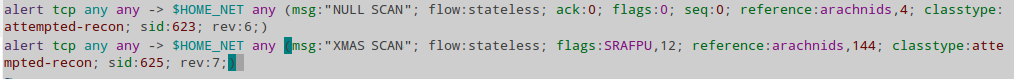
\includegraphics[width= 1\linewidth]{../images/VM_XMAS_2.png}
\end{figure}
\end{frame}
\begin{frame}
\frametitle{Portscans - NULL and XMAS (2/2)}
\textbf{nmap -T4 -A -sN -sX -v 192.168.100.17}. \\
Now everything works fines
\begin{figure}
   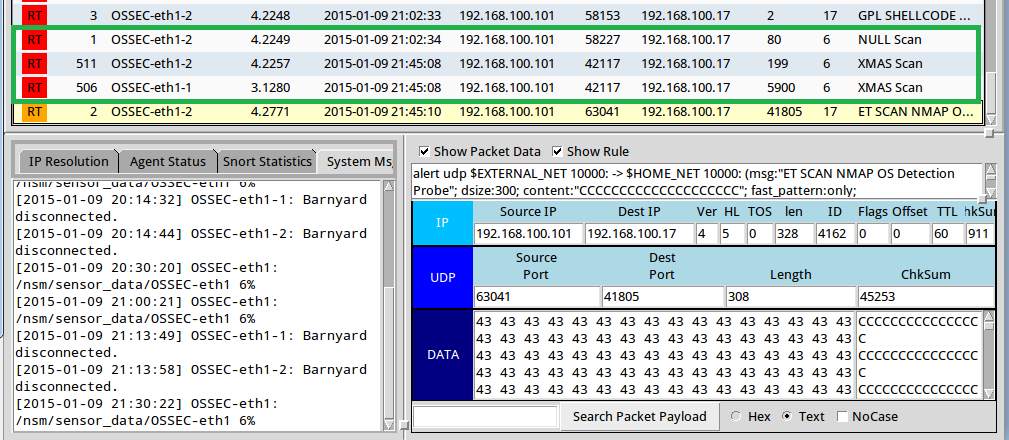
\includegraphics[width= 1\linewidth]{../images/VM_XMAS.png}
\end{figure}
\end{frame}

%---------------------------------

\begin{frame}
\frametitle{Webserver attacks - XSS (1/3)}
Custom-made vulnerable webpage
\begin{figure}
   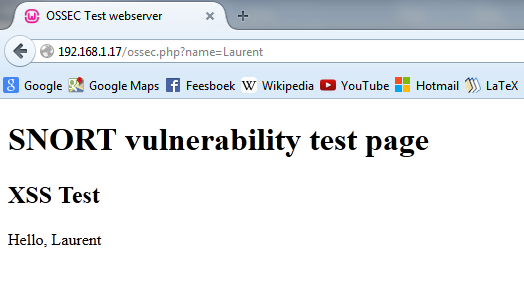
\includegraphics[width= 0.7\linewidth]{../images/VM_XSS_1.png}
\end{figure}
\end{frame}
\begin{frame}
\frametitle{Webserver attacks - XSS (2/3)}
\textbf{$<$script$>$alert('XSS vulnerability')$<$/script$>$}.
\begin{figure}
   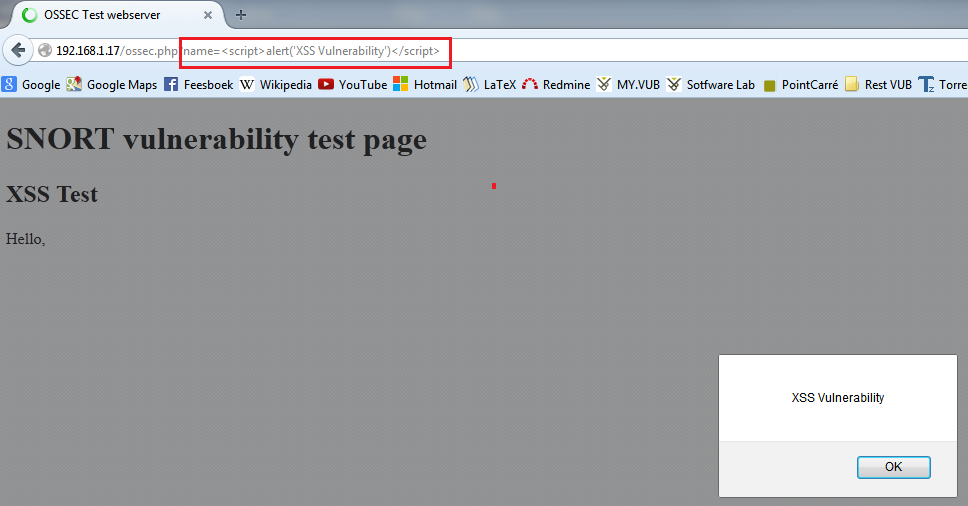
\includegraphics[width= 0.8\linewidth]{../images/VM_XSS_2.png}
\end{figure}
\end{frame}
\begin{frame}
\frametitle{Webserver attacks - XSS (3/3)}
Detected by Snort!
\begin{figure}
   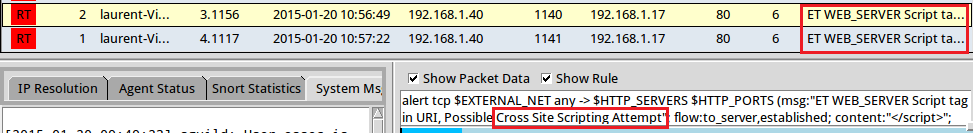
\includegraphics[width= 1\linewidth]{../images/VM_XSS_5.png}
\end{figure}
But can we prevent this attack?
\begin{figure}
   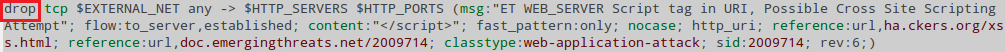
\includegraphics[width= 1\linewidth]{../images/VM_XSS_6.png}
\end{figure}
\end{frame}

%---------------------

\begin{frame}
\frametitle{Webserver attacks - VISA Card number sent in plain text over network (1/3)}
Not supported by Snort $=>$ need to add our own rule
\begin{figure}
   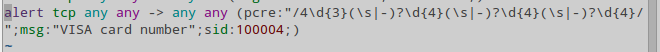
\includegraphics[width= 1\linewidth]{../images/VM_VISA.png}
\end{figure}
\end{frame}
\begin{frame}
\frametitle{Webserver attacks - VISA Card number sent in plain text over network (2/3)}
Custom webpage to insert VISA Card number
\begin{figure}
   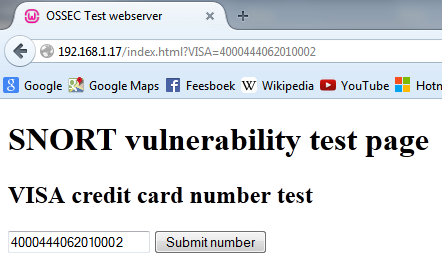
\includegraphics[width= 0.6\linewidth]{../images/VM_VISA_2.png}
\end{figure}
\end{frame}
\begin{frame}
\frametitle{Webserver attacks - VISA Card number sent in plain text over network (3/3)}
Detected by Snort!
\begin{figure}
   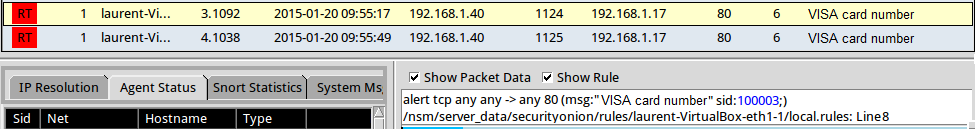
\includegraphics[width= 1\linewidth]{../images/VM_VISA_3.png}
\end{figure}
Without the rules, this would not be possible!
\end{frame}
%-------------------------

\begin{frame}
\frametitle{FTP server attacks - Root access (1/2)}
Not supported by Snort $=>$ need to add our own rule
\begin{figure}
   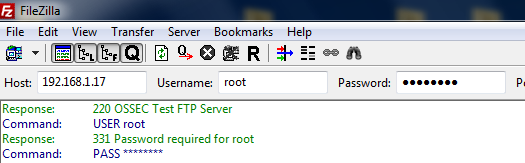
\includegraphics[width= 0.7\linewidth]{../images/VM_FTP_3.png}
\end{figure}
\end{frame}
\begin{frame}
\frametitle{FTP server attacks - Root access (2/2)}
Not supported by Snort $=>$ need to add our own rule\ldots
\begin{figure}
   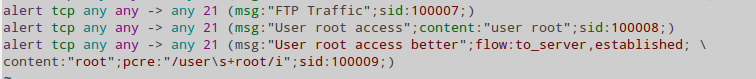
\includegraphics[width= 1\linewidth]{../images/VM_FTP_2.png}
\end{figure}
\ldots after which Snort alerts properly.
\begin{figure}
   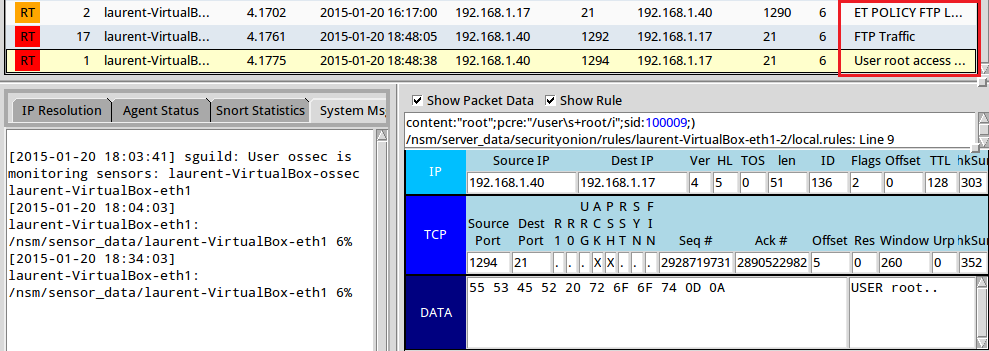
\includegraphics[width= 1\linewidth]{../images/VM_FTP_4.png}
\end{figure}
\end{frame}
\begin{frame}
\frametitle{FTP server attacks - attacks using Metasploit (1/2)}
\textbf{Let's go into more serious stuff\ldots}
\begin{figure}
   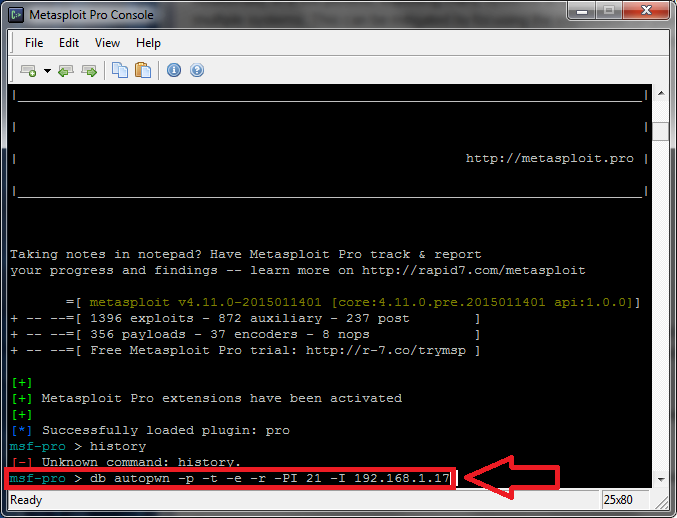
\includegraphics[width= 0.7\linewidth]{../images/VM_FTP_8.png}
\end{figure}
\end{frame}
\begin{frame}
\frametitle{FTP server attacks - attacks using Metasploit (2/2)}
\begin{figure}
   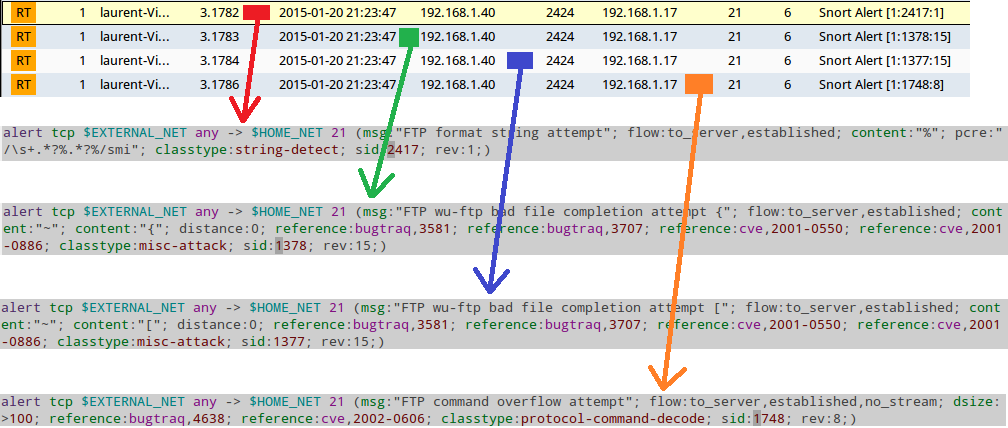
\includegraphics[width= 1\linewidth]{../images/VM_FTP_7.png}
\end{figure}
Without those rules, this would not be possible!
\end{frame}
%--------------------------------------------------------------------

\begin{frame}
\frametitle{SSH server attacks - attacks using Metasploit (1/3)}
\begin{figure}
   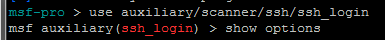
\includegraphics[width= 0.6\linewidth]{../images/VM_SSH_3.png}
\end{figure}
Load the file containing the usernames and passwords \ldots
\begin{figure}
   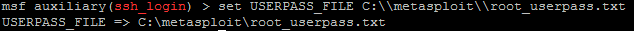
\includegraphics[width= 0.9\linewidth]{../images/VM_SSH_4.png}
\end{figure}
\ldots configure some other options \ldots
\begin{figure}
   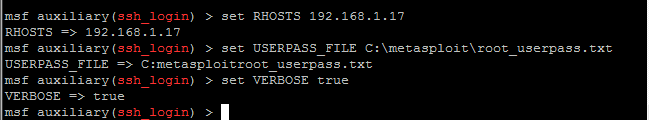
\includegraphics[width= 0.9\linewidth]{../images/VM_SSH_2.png}
\end{figure}
\end{frame}
\begin{frame}
\frametitle{SSH server attacks - attacks using Metasploit (2/3)}
\ldots and begin the attack!
\begin{figure}
   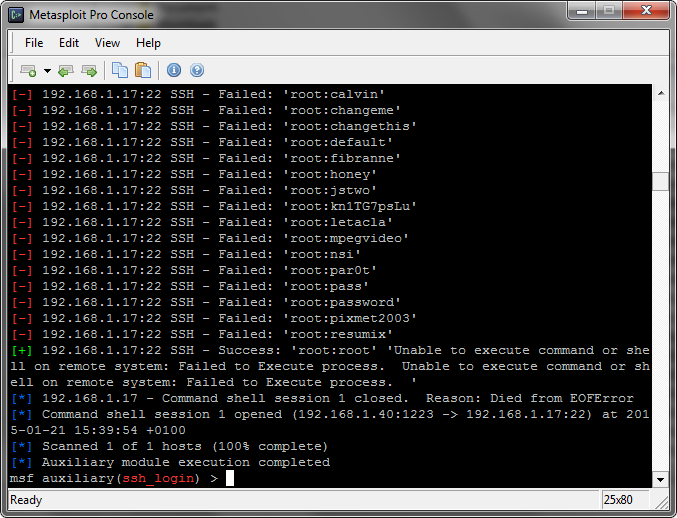
\includegraphics[width= 0.7\linewidth]{../images/VM_SSH_5.png}
\end{figure}
The bruteforcing in action\ldots
\end{frame}
\begin{frame}
\frametitle{SSH server attacks - attacks using Metasploit (3/3)}
Detected by Snort out-of-the-box.
\begin{figure}
   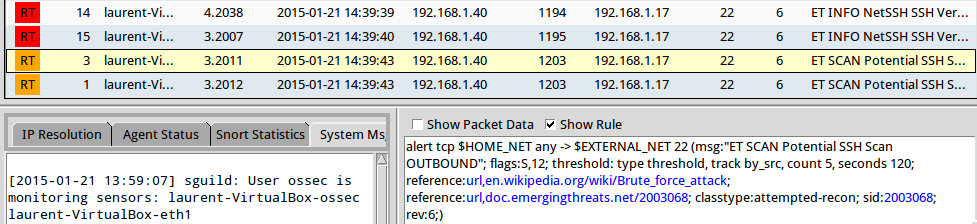
\includegraphics[width= 1\linewidth]{../images/VM_SSH_6.png}
\end{figure}
\end{frame}

%--------------------------------------------------------------------
\begin{frame}
\frametitle{Database attacks (1/2)}
Rules to detect root access and executing some commands
\begin{figure}
   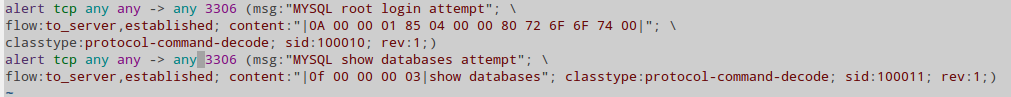
\includegraphics[width= 1\linewidth]{../images/VM_MSSQL_5.png}
\end{figure}
\begin{figure}
   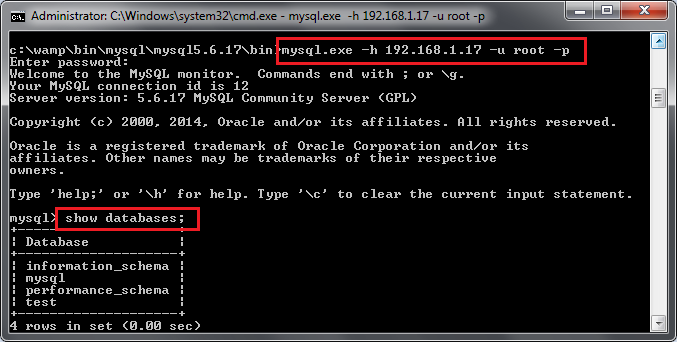
\includegraphics[width= 0.7\linewidth]{../images/VM_MSSQL_4.png}
\end{figure}
\end{frame}
\begin{frame}
\frametitle{Database attacks (2/2)}
Detected by Snort!
\begin{figure}
   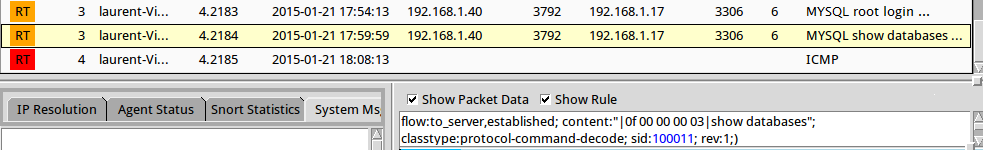
\includegraphics[width= 1\linewidth]{../images/VM_MSSQL_6.png}
\end{figure}
Without the rules, this would not have been detected!
\end{frame}


%--------------------------------------------------------------------

\begin{frame}
\frametitle{Trojan injection / infection (1/4)}
Create the trojan\ldots
\begin{figure}
   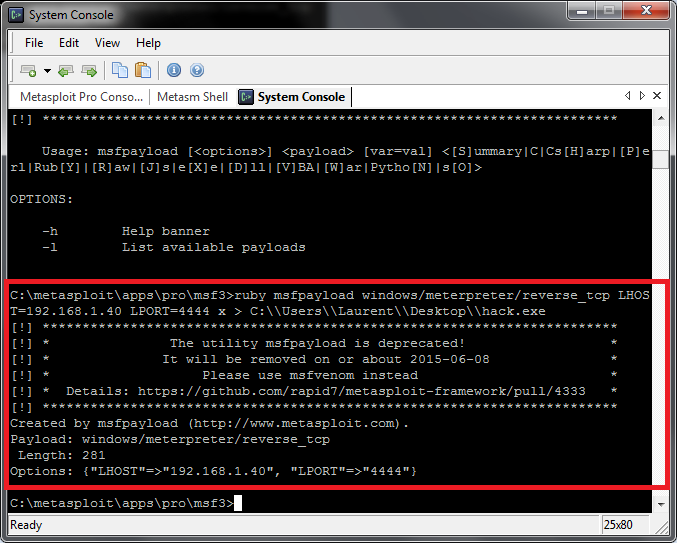
\includegraphics[width= 0.5\linewidth]{../images/VM_Trojan_2.png}
\end{figure}
\begin{figure}
   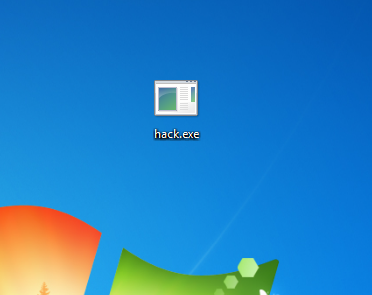
\includegraphics[width= 0.3\linewidth]{../images/VM_Trojan_6.png}
\end{figure}
\end{frame}
\begin{frame}
\frametitle{Trojan injection / infection (2/4)}
\ldots setup the listener \ldots
\begin{figure}
   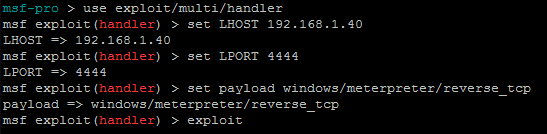
\includegraphics[width= 0.7\linewidth]{../images/VM_Trojan_3.png}
\end{figure}
\end{frame}
\begin{frame}
\frametitle{Trojan injection / infection (3/4)}
\ldots and wait.
\begin{figure}
   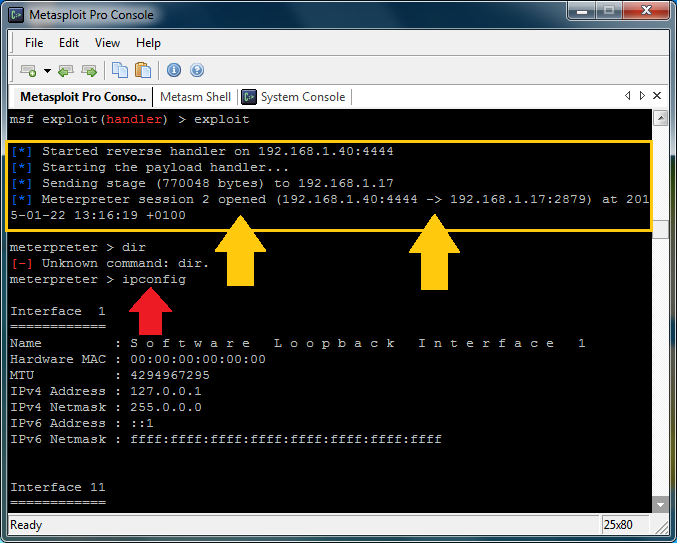
\includegraphics[width= 0.4\linewidth]{../images/VM_Trojan_5.png}
\end{figure}
\begin{figure}
   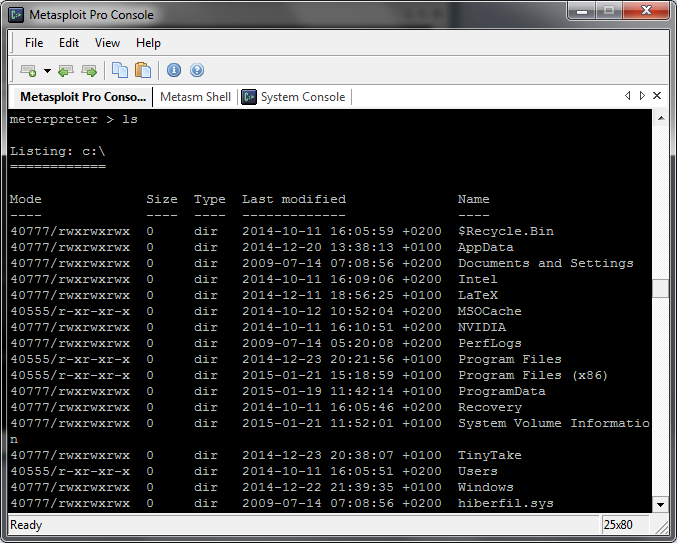
\includegraphics[width= 0.4\linewidth]{../images/VM_Trojan_4.png}
\end{figure}
\end{frame}
\begin{frame}
\frametitle{Trojan injection / infection (4/4)}
Detected by Snort!
\begin{figure}
   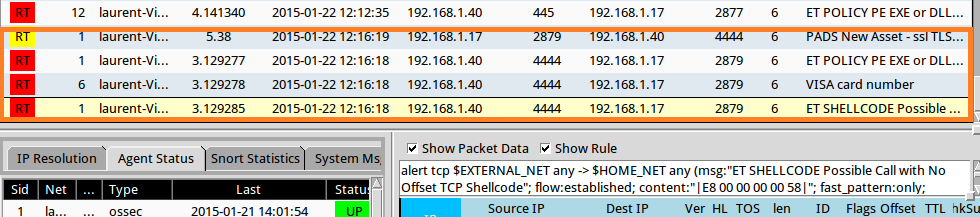
\includegraphics[width= 1\linewidth]{../images/VM_Trojan_1.png}
\end{figure}
\end{frame}

%---------------------------------------------------------------------

\section{Additional configuration}
\subsection*{}

\begin{frame}
\frametitle{\insertsection}
\textbf{Additional configuration and fine-tuning Snort}
\end{frame}

\begin{frame}
\frametitle{Classifying alerts - manually}
By pressing function keys in the realtime viewer of Sguil.
\begin{enumerate}
\item F1: Category I: Unauthorized Root/Admin access.
\item F2: Category II: Unauthorized User access.
\item F3: Category III: Attempted Unauthorized Access
\item F4: Category IV: Successful Denial-of-Service Attack
\item F5: Category V: Poor Security Practice or Policy Violation
\item F6: Category VI: Reconnaissance/Probes/Scans
\item F7: Category VII: Virus Infection
\item F8: No action necessary
\end{enumerate}
\begin{figure}
   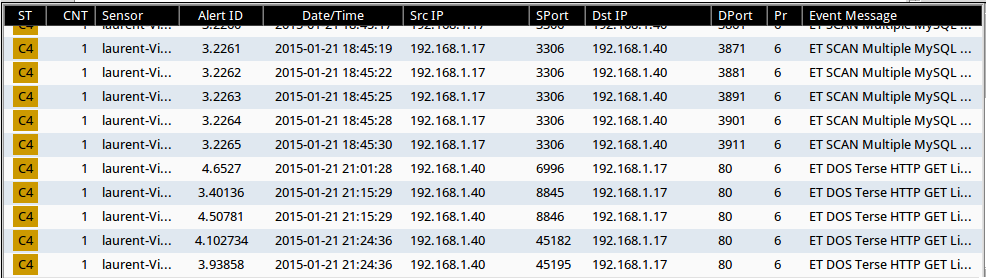
\includegraphics[width= 0.7\linewidth]{../images/VM_CAT_4.png}
\end{figure}
\end{frame}

\begin{frame}
\frametitle{Classifying alerts - automatically}
By editing \textbf{autocat.conf}.
\begin{figure}
   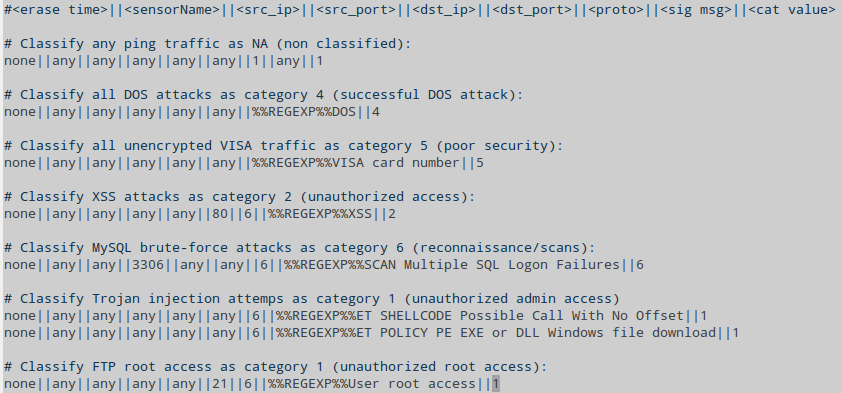
\includegraphics[width= 1\linewidth]{../images/VM_CAT_7.png}
\end{figure}
\end{frame}

\begin{frame}
\frametitle{Fine-tuning rules}
Set thresholds and suppress rules
\begin{figure}
   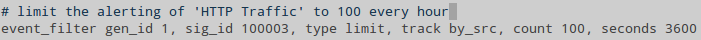
\includegraphics[width= 1\linewidth]{../images/VM_DB_8.png}
\end{figure}
\begin{figure}
   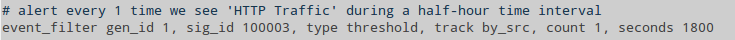
\includegraphics[width= 1\linewidth]{../images/VM_DB_9.png}
\end{figure}
\begin{figure}
   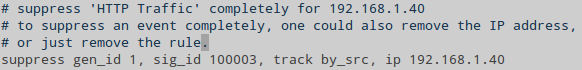
\includegraphics[width= 1\linewidth]{../images/VM_DB_10.png}
\end{figure}
\end{frame}

\begin{frame}
\frametitle{False alerts}
Eliminate false alerts
\begin{figure}
   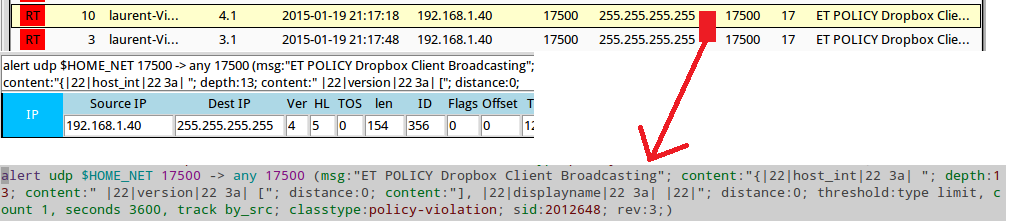
\includegraphics[width= 1\linewidth]{../images/VM_Dropbox.png}
\end{figure}
\end{frame}


%---------------------------------------------------------------------

\section{Conclusions}
\subsection*{}

\begin{frame}
\frametitle{Difficulties}
\begin{block}{Difficulties encountered}
\begin{itemize}
\item Installing Snort
\item Configuring Snort
\item Sometimes the agent won't start
\item Logfile analysis
\item \ldots
\end{itemize}
\end{block}
\end{frame}

\begin{frame}
\frametitle{Conclusion}
\begin{block}{Findings and conclusion}
\begin{itemize}
\item Out-of-the-box: mediocre
\item Rules have to be added/modified/deleted
\item Takes a lot of time to configure
\item Very extendable
\item Very capable once correctly configured
\end{itemize}
\end{block}
\end{frame}

\begin{frame}
\frametitle{End}
QA time
\end{frame}

\end{document} 